	\documentclass{article}
\usepackage[utf8]{inputenc}
\usepackage{graphicx}
\usepackage[margin=2.5cm]{geometry}
\usepackage{eso-pic}
\usepackage{hyperref}
\usepackage{wrapfig}
\usepackage{lipsum}
\usepackage{array}
\usepackage{enumitem}
\AddToShipoutPictureBG{%
    \AtPageLowerLeft{
        % \hspace{1cm}
        
\includegraphics[width=4.5cm]{img/Java-Hutts2.png}
    }
}
\title{Architectural Design Specification}
\date{2017}
\def \project{Electronic ID Verification }
\begin{document}

\makeatletter
    \begin{titlepage}
        \begin{center}
            
\includegraphics[width=0.7\linewidth]{img/up.png}\\[4ex]
            {\huge \bfseries \@title }\\[2ex]
            {\LARGE \textbf{Team:} Java the Hutts}\\[2ex]
            {\LARGE \@date}\\[2ex]
            {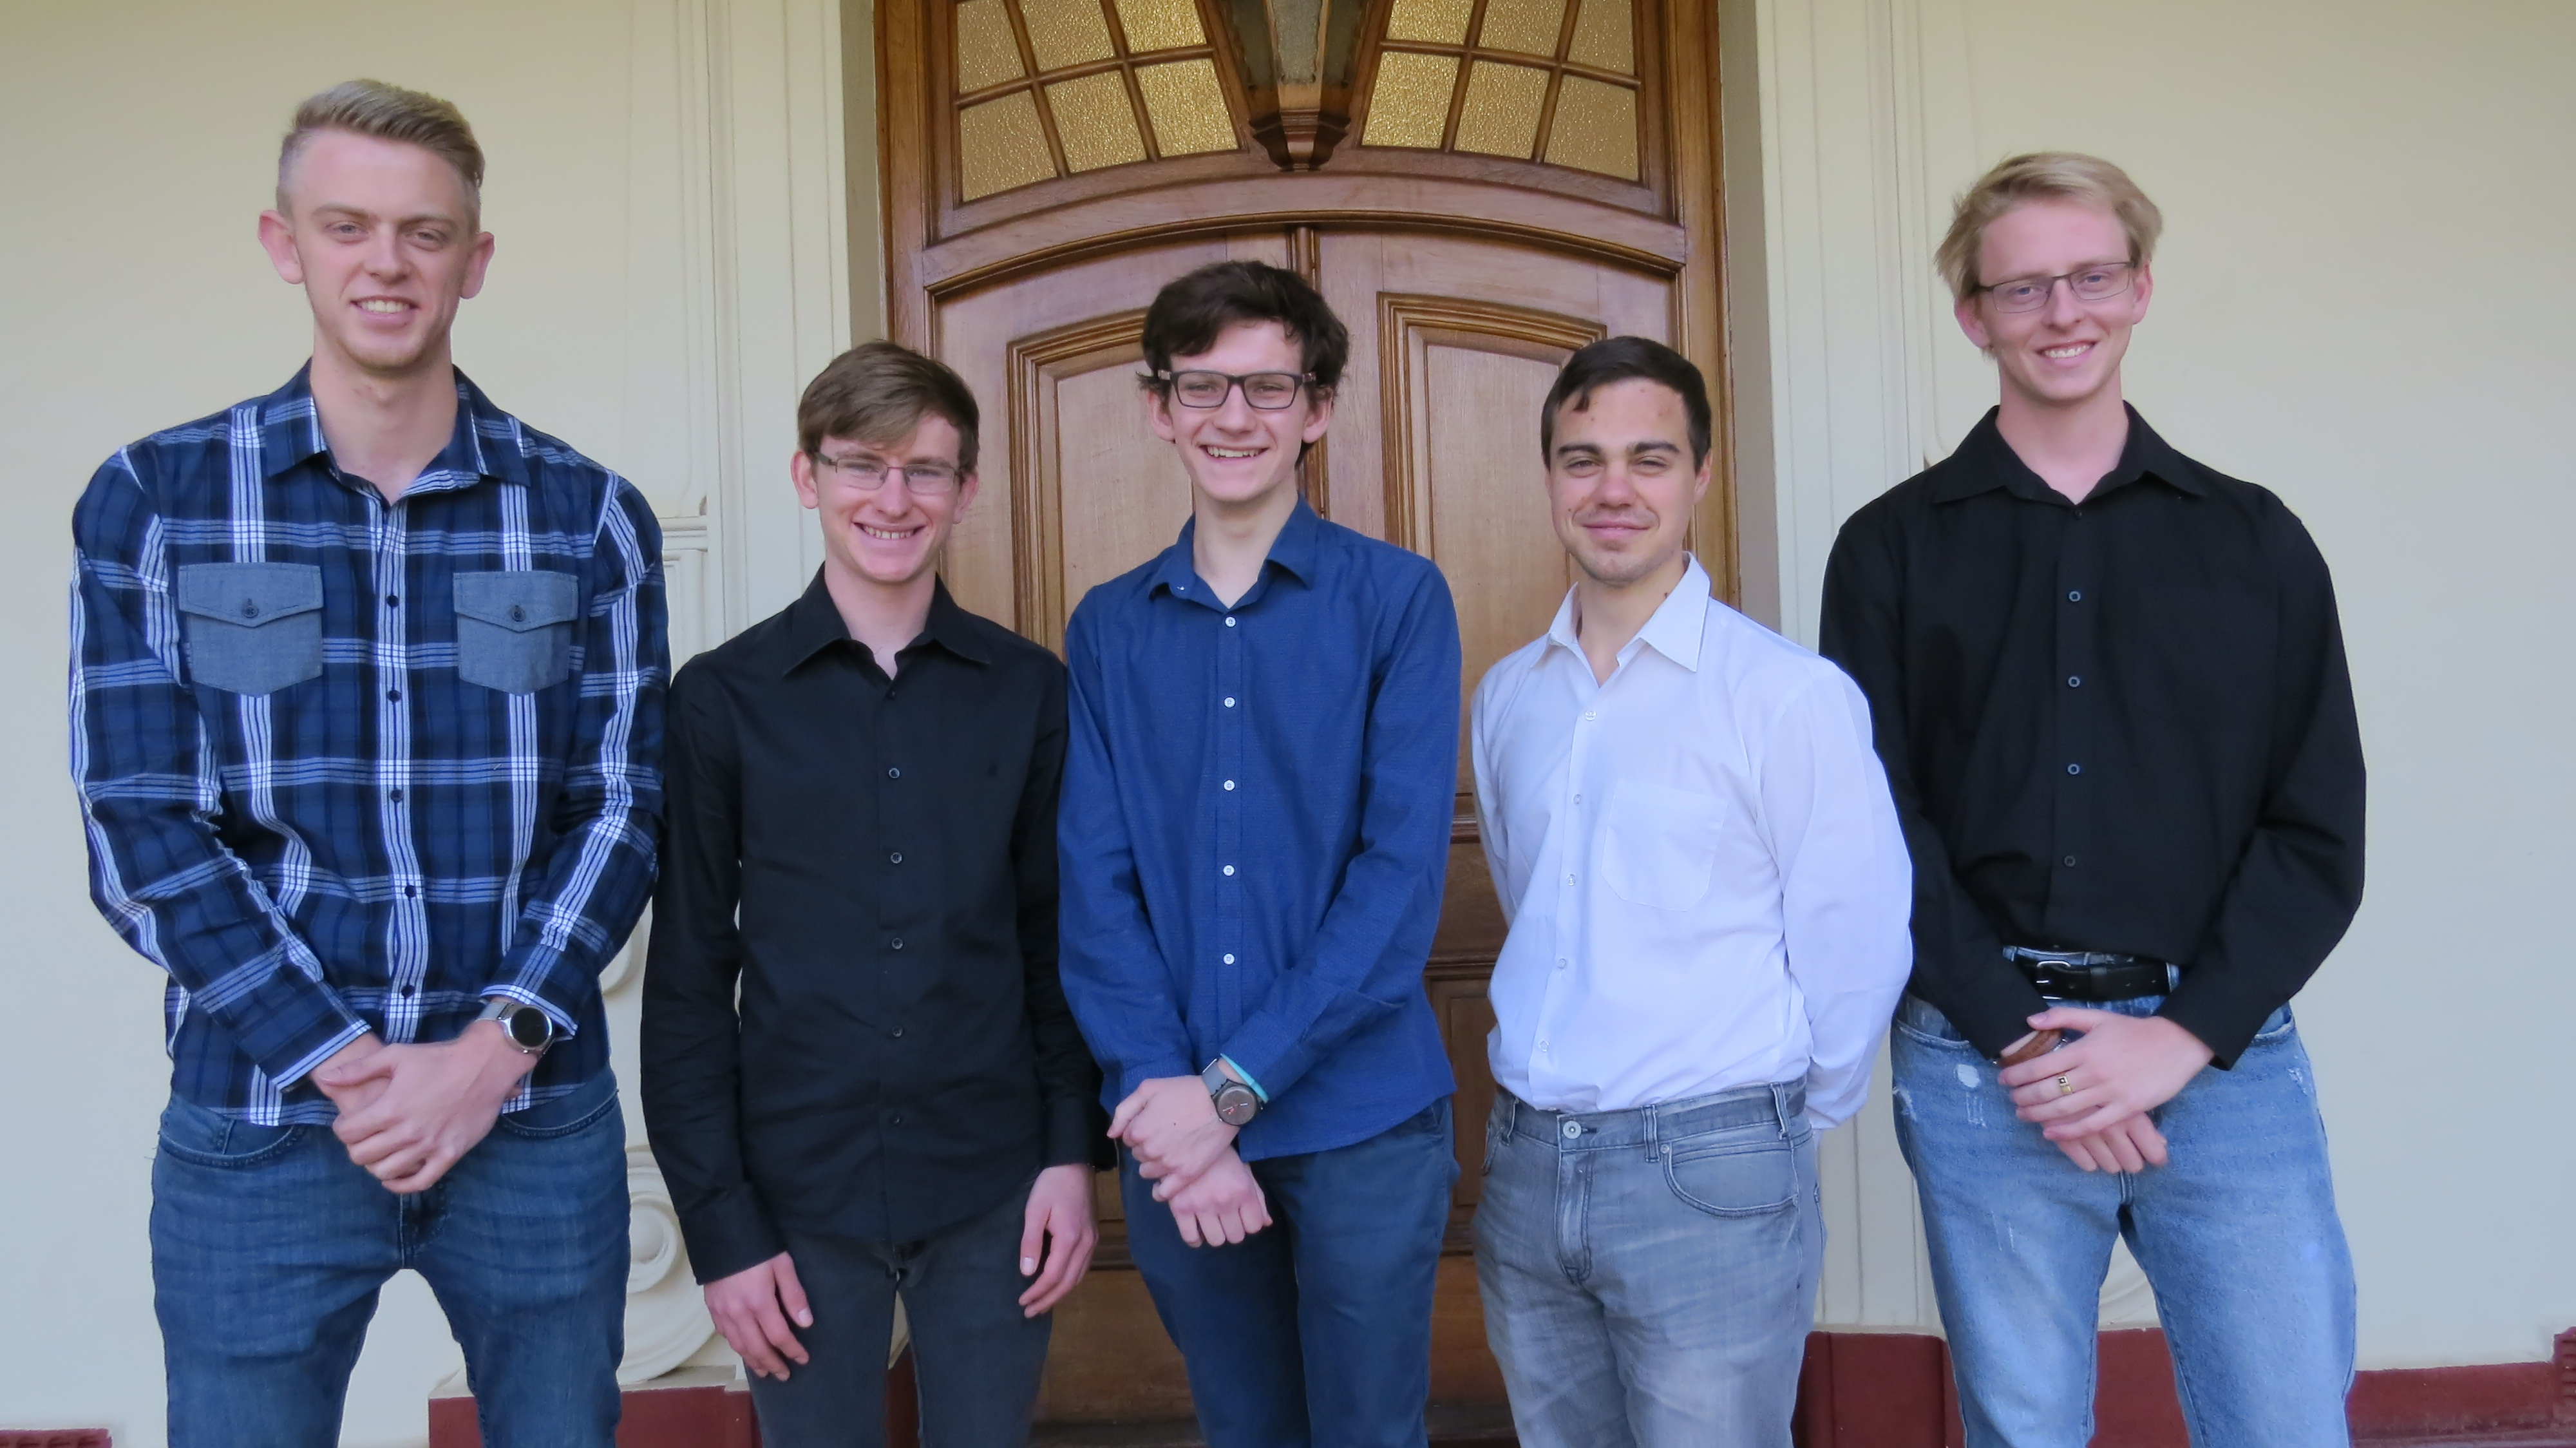
\includegraphics[width=\linewidth]{img/team_photo.jpg}}\\[2ex]
            {\large  Nicolai van Niekerk\\ \texttt{nicvaniek@gmail.com}}\\[2ex]
            {\large  Marno Hermann\\ \texttt{marno@barnton-consulting.co.za}}\\[2ex]
            {\large  Stephan Nell\\ \texttt{nellstephanj@gmail.com}}\\[2ex]
            {\large  Jan-Justin van Tonder\\ \texttt{J.vanTonder@tuks.co.za}}\\[2ex]
            {\large  Andreas Nel\\ \texttt{nel.andreas1@gmail.com}}\\[2ex]
        \end{center}
        
    \end{titlepage}
\makeatother

\cleardoublepage
\thispagestyle{empty}
\tableofcontents
\newpage

\setcounter{page}{1}
	\section{Architectural Specifications and Design}\label{sec:architectural}
	The purpose of this document is to give an architectural perspective of the \project system through the use of various visual models. The models depict the components of the \project system where appropriate. Additionally, the various technologies that are implemented will be addressed.
	
	    \subsection{Deployment Model}\label{sec:architectural-deployment}
	    The following Deployment diagram depicts the architecture of the system as deployment of artifacts to deployment targets.
	    \begin{figure}[h]
	    	\centering
	    	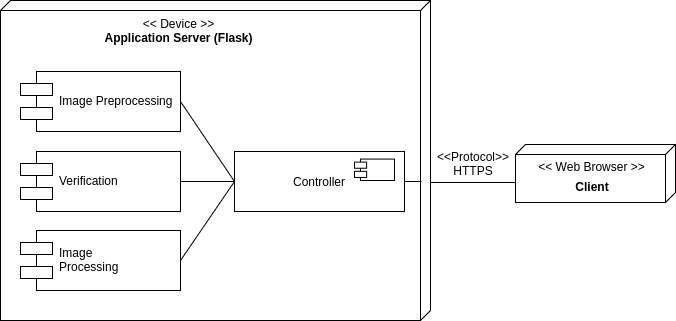
\includegraphics[scale=0.5]{img/Quant.png}
	    	\caption{Deployment Diagram}
	    \end{figure}
	    
	    \subsection{Use Case Models}\label{sec:architectural-use-case}
	    
	    \subsection{Class Models}\label{sec:architectural-class}
	    
	    \subsection{Activity Models}\label{sec:architectural-activity}
	    
	    \subsection{Sequence Models}\label{sec:architectural-sequence}
	    
	    \subsection{State Models}\label{sec:architectural-state}
	    
	    \subsection{Technologies}\label{sec:architectural-technologies}
	    \end{document}